% !TeX root = ../../main.tex

\subsection{拆装步骤及操作方式}
\subsubsection{脉冲器拆装步骤及操作方式}
1）下井前准备

(1) 了解井况，确定套管或者管径规格和深度等基本信息；

(2) 确定工具活动部件是否连接稳固，外观是否存在不合格如裂纹缺口问题，如出现，则不能入井；

(3) 确定工具和其余钻具的连接扣型是否正确；

(4) 可按照推荐排量在井台上检验工具是否能正常振动，喷水口严禁对人。

2）操作方法

(1) 核准下井油管尺寸；

(2) 用“通井规”通井、洗井，若和其他具有通、洗井功能的工具配合使用时可一体化完成；

(3) 将工具缓慢下至设计位置；

(4) 连接管线等地面加压设备后试压；

(5) 开泵加压、冲洗井底，推荐的排量为100L/min-500L/min（直至上返水无污物止）；

(6) 控制出口流量，加大井口压力、排量到设计压力、排量进行正常振动作业；

(7) 每振动1小时，停振10分钟，累计振动作业4-6小时停振、泄压、将工具取出。

3）注意事项

(1) 工具与管柱的连接扣必须拧紧。

(2) 公扣端需要朝下。

(3) 脉冲器在下入过程中如遇阻，应慢慢旋转几圈后再下放。

(4) 不能连续振动超过十分钟。

\subsubsection{旋转喷头拆装步骤及操作方式}

\subsubsubsection{拆卸}

准备工具：3mm + 4mm内六方扳手、3/8\inch 套筒、套筒扳手、卸扣工装、可调扳手、链钳\footnote{注：重要！工具需夹紧在装配钳台上。}

\begin{itemize}
	\item 取出筒体2上螺钉
	
	\begin{figure}[htbp]
		\centering
		\includegraphics[width=0.5\textwidth]{figure/chapter3/part1-3in1/nozzle-unsetup-step1.png}
		%\caption{拆卸步骤1：取出筒体2上螺钉}
		\label{fig:unscrew_from_body2}
	\end{figure}	
 
		\item 从筒体2上卸掉上接头1和波簧15
\begin{figure}[htbp]
	\centering
	\includegraphics[width=0.5\textwidth]{figure/chapter3/part1-3in1/nozzle-unsetup-step2.png}
	%\caption{拆卸步骤2：卸掉上接头1和波簧15}
	%\label{fig:unscrew_from_body2}
\end{figure}
 
		\item 从上接头1上取出骨架油封7，密封垫环21，卸掉带孔螺钉19取出O型圈31。
\begin{figure}[htbp]
	\centering
	\includegraphics[width=0.7\textwidth]{figure/chapter3/part1-3in1/nozzle-unsetup-step3.png}
	%\caption{拆卸步骤3：取出骨架油封7、密封垫环21与O型圈31}
	%\label{fig:unscrew_from_body2}
\end{figure}
 
		\item 从本体2上卸掉底部帽，取下轴承12和隔套13。
	\begin{figure}[htbp]
		\centering
		\includegraphics[width=0.7\textwidth]{figure/chapter3/part1-3in1/nozzle-unsetup-step4.png}
		%\caption{拆卸步骤4：卸掉底部帽，取下轴承12和隔套13}
		%\label{fig:unscrew_from_body2}
	\end{figure}
	
	\item 先从旋转头16上卸掉紧定螺钉34，然后将旋转头16从喷头连接体10上卸下来。然后再将紧定螺钉33从喷头连接体10上卸下来，最后将喷头连接体10从心轴4上卸下来。
	\begin{figure}[htbp]
		\centering
		\includegraphics[width=0.7\textwidth]{figure/chapter3/part1-3in1/nozzle-unsetup-step5.png}
		%\caption{拆卸步骤5：卸下旋转头16与喷头连接体10}
		%\label{fig:unscrew_from_body2}
	\end{figure}
	
 
	\item 从心轴4上卸掉底部帽8和轴承12，插入座3和O型圈26。
	\begin{figure}[htbp]
		\centering
		\includegraphics[width=0.7\textwidth]{figure/chapter3/part1-3in1/nozzle-unsetup-step6.png}
		%\caption{拆卸步骤6：卸掉底部帽8和轴承12，取出插入座3与O型圈26}
		%\label{fig:unscrew_from_body2}
	\end{figure}
	
 
	\item 从底部帽8上卸掉平衡活塞座9，取出大弹簧20和O型圈28，取出平衡活塞6。
	\begin{figure}[htbp]
		\centering
		\includegraphics[width=0.7\textwidth]{figure/chapter3/part1-3in1/nozzle-unsetup-step7.png}
		%\caption{拆卸步骤7：卸掉平衡活塞座9，取出大弹簧20、O型圈28与平衡活塞6}
		%\label{fig:unscrew_from_body2}
	\end{figure}
 
	\item 从喷头连接体10上取出O型圈29和30。从平衡活塞上取出骨架油封7和O型圈27。
		\begin{figure}[htbp]
		\centering
		\includegraphics[width=0.7\textwidth]{figure/chapter3/part1-3in1/nozzle-unsetup-step8.png}
		%\caption{拆卸步骤8：取出O型圈29、30与骨架油封7}
		%\label{fig:unscrew_from_body2}
	\end{figure}
 
	\item 从旋转喷头16上取下喷嘴18，从隔套13上取出连通隔套5。
	\begin{figure}[htbp]
		\centering
		\includegraphics[width=0.7\textwidth]{figure/chapter3/part1-3in1/nozzle-unsetup-step9.png}
		%\caption{拆卸步骤9：取下喷嘴18与连通隔套5}
		%\label{fig:unscrew_from_body2}
	\end{figure}
	
\item 	准备清洗和检测。
	
\end{itemize}
	
\subsubsubsection{装配}
准备工具：3mm+4mm内六方扳手、3/8\inch 套筒、套筒扳手、扣工装、可调扳手、链钳\footnote{注：重要！工具需夹紧在装配钳台上。}。装配前，检查所有部件是否磨损和腐蚀；润滑所有密封区域并安装O型圈/支撑环。涂抹润滑脂润滑所有螺纹防止粘扣。
\begin{itemize}
	\item 在喷头连接体10上安装O型圈29和O型圈30，在平衡活塞6上安装骨架油封7和O型圈27。
	
	\item 在旋转喷头16上安装喷嘴和引流体17。
	
	\item 在底部帽8上安装O型圈28并依次装入已经小装好的平衡活塞6和大弹簧20和平衡活塞座9。
	
	\item 在心轴4上安装O型圈26和插入座3，掉头将两件轴承12装入心轴4并将底部帽8和心轴连接到位。
	
	\item 将小装好的喷头连接体10和小装好的心轴4连接到位，并将紧定螺钉33安装在喷头连接体10上。然后将小装好的旋转喷头16和喷头连接体10连接到位后，将紧定螺钉34安装在旋转喷头上。
	
	\item 将底部帽8和筒体2连接到位，在筒体上安装紧定螺钉32，将连通隔套5和隔套13安装，依次将小装后的隔套13、轴承12、波簧15装入筒体2。确保连通隔套5和心轴4的限位台阶抵紧。
	
	\item 在上接头1上安装O型圈25，O型圈31和带孔螺钉19，并依次在上接头1上装入骨架油封7和密封垫环21。
	
	\item 将装好的上接头1和小装好的筒体2连接到位后安装紧定螺钉32。
	
	\item 安装好之后注油进行旋转测试。
\end{itemize}
	
	
\subsubsubsection{注油}

准备工具：3mm + 4mm内六方扳手、可调扳手、链钳\footnote{
注（重要）：工具需夹紧在装配钳台上。}

\begin{itemize}

	\item 从筒体2上取掉紧定螺钉32，然后将上接头1从筒体2上卸下来。
	\item 保持旋转喷嘴直立，使用混合硅胶油-1000，直到油位位于筒体2的槽螺孔下方。
 
注：建议让喷嘴直立过夜，使油沉淀。回装喷嘴时，可能需要补注摩擦螺钉下方的油。

	\item 将上接头1和筒体2连接至0.31\inch（7.87 mm），卸掉带孔螺钉19继续上扣至紧扣扭矩。
	
	\item 在筒体2上安装好带孔螺钉19和紧定螺钉32。
 
	\item 安装喷嘴后准备测试。
	\end{itemize}
	
\subsubsubsection{功能测试}
\begin{itemize}
	
	\item 充油后目视检查工具，检查在修整过程中是否有泄漏或任何密封件损坏。
	
	\item 用手旋转工具，确保其转动平稳，不过度用力，不干涉。
	
	\item 将工具连接到泵上，并开始以最低速率循环通过泵，逐渐增加速率，直到它开始旋转并记录流量。
	
	\item 继续观察恒定流速下是否出现泄漏情况，如果观察到任何泄漏，请参考总装图，以确定哪个密封/密封正在通过。应注意，该工具存在内置的泄漏路径，允许流体通过外壳离开工具。
	
	\item 通常，所有尺寸的工具都会开始以小于0.6次/分的速度旋转，具体值可能存在差异，这取决于心轴上新唇密封的实际配合状态。如果启动旋转所需的流量高于预期，建议增加流量5$\sim$10 L/min；当新唇密封磨损后，应停止泵送并重复上述操作。
	
	\item 如果不能以所需的流量启动旋转，建议将驱动旋转的两个90度喷嘴更换成更大孔径的喷嘴，以允许喷嘴的流量比例更大。
	\end{itemize}
	
\subsubsubsection{操作方法}
	\begin{itemize}
		
	\item 该工具可以单独用于清洗油套管，也可以和其他工具组合作业。
	
	\item 将旋转头下入井内距离清洁位置1$\sim$3 m处，开泵循环，排量建议为100 L/min，逐渐加大流量但最大不应超过300 L/min。同时若配置其他工具，需要保持稳定的循环，平稳地上下活动钻具。
	
	\item 起钻时要求平稳、低速、严禁剧烈振动与撞击。
	\end{itemize}

\subsubsection{液压刮管器拆装步骤及操作方式}

\subsubsubsection{下井前准备}
		\begin{itemize}
		\item 了解井况，确定套管规格和深度等基本信息；
		\item 根据刮管工艺要求，确定套管是否需要液压启动后再进行刮管。
		\end{itemize}
	
\subsubsubsection{操作方法}
\begin{itemize}
	\item 下井前按作业要求依次连接好管柱，刮管器前端需接与套管规格对应的扶正器；推荐管柱组合：通井钻头+扶正器+液压刮管器+上部钻柱；
	\item 接上刮管器后，夹紧下接头，用大钳咬住上接头，拧紧刮管器各连接螺纹；
	\item 需要进行刮管作业时，将刮管器下入到所需的井深位置后，投入钢球，开泵进行打压启动作业；其中，刮管器打开压力$=$静液柱压力$+$泵压（绝对压力），即泵压$\ge$绝对压力$-$静液柱压力；
	\item 观察泵压有下降后，说明刮管器启动，此时通过上提、下放工具，如此反复进行刮管作业；
	\item 刮管作业中观察指重表无任何显示，即下放悬重不降、上提悬重不升，表明已刮削干净；
	\item 若上提过程中多次遇阻仍无法上提，可投入复位钢球，开泵将刮刀体强行收回；
	\end{itemize}
\subsubsubsection{注意事项}
	\begin{itemize}
		\item 工具与管柱的连接扣必须拧紧。
		\item 刮管器在下井过程中如遇阻，应慢慢旋转几圈后再下放。
		\item 刮削过程中，必须始终保持循环畅通。
	\end{itemize}
\subsubsection{毛刷刮管器拆装步骤及操作方式}
\subsubsubsection{拆卸}\label{sec:unstep_swiper}
	\begin{itemize}
	\item 去掉防掉螺钉后，用拧扣机拆卸下接头；
	\item 依次取出心轴上的上扶正套、毛刷体、下扶正套、剪切套、剪切定位套；
	\item 取出所有O型圈与销钉。
	\item 零部件清洗，打磨处理工具表面锈蚀部分；
	\item 清洗并晾干所有零部件。
	\end{itemize}
\subsubsubsection{装配}
按照\ref{sec:unstep_swiper}所述“拆卸”步骤的反序组装各部件。注意：
\begin{itemize}
	\item 所有密封圈及工具配合面涂润滑油，上扶正套、毛刷体、下扶正套、剪切套、剪切定位套与心轴间涂抹黄油；
	\item 产品连接螺纹涂钻具螺纹脂；
	\item 上、下接头的上扣扭矩为$10\ \mathrm{kN\cdot m}$；
	\item 产品本体喷涂天蓝色脂肪族面漆，毛刷喷银色漆；
	\item 两端接头螺纹涂防蚀脂并佩戴护丝。
	\end{itemize}
\subsubsubsection{使用方法}
\begin{itemize}
	\item 	根据井眼尺寸选择合适的套管刮管器。
	\item 套管刮管器用钻柱送入井底进行刮管作业，情况允许也可以用钢丝绳或者连续油管送入。
\end{itemize}
\subsubsubsection{操作方法}
\begin{itemize}
	\item 	该工具可以与液压刮管器以及强磁打捞器配合使用，也可以在刮完井之后使用。
	\item 	将套管刮管器下到井底离通井位置3$\sim$5 m处，开泵循环。将套管刮管器在该位置上下活动，保持循环的情况下平稳地上提钻柱。
	\item 	起钻时要求平稳、低速、严禁剧烈振动与撞击。
\end{itemize}

\subsection{注意事项}

\begin{itemize}
	\item 脉冲器与管柱的连接扣必须拧紧，公扣端朝下；下入过程中如遇阻，应慢慢旋转几圈后再下放；
	单次连续振动不得超过 10\,min，累计振动每满 1\,h 应停振 10\,min 散热。
	\item 液压刮管器与管柱的连接扣必须拧紧，下井过程中如遇阻应慢慢旋转几圈后再下放，刮削过程中必须
	始终保持循环畅通；起钻前先停泵泄压并确认刮刀收回。
	\item 一趟管柱内同时使用多种液压启动工具时，应预先确定投球顺序与憋压值，避免先投球激活的工具
	影响后续工序。
\end{itemize}

\subsection{三个模块的疲劳寿命有限元分析}
三合一工具的脉冲短节、毛刷刮管器与液压刮管器按同一额定载荷 400\,kN 与 400\,kN 级扭矩评定，
额定值低于其余四款工具，承力截面尺寸也相应偏小。三者的材料档不同：脉冲短节为 4145 的 827/965 档
（$\sigma_a=3\,752\,N^{-0.2189}$），毛刷刮管器与液压刮管器的承力件为 4145H 的 825/965 档
（$\sigma_a=3\,840\,N^{-0.2227}$，$1\times10^{6}$ 次处 177.2\,MPa）。

计算方法与第 1 章一致：$R=0$ 脉动循环，Goodman 修正，设计循环数 1\,000 次；
峰值应力位于接触终止线，不参与评定，评定值取距峰值数毫米、梯度趋平缓处的节点应力。
液压刮管器按四件整体建模（上接头、本体、连接体、下接头），上接头 NC31 Box 端面固定，
下接头 NC31 Pin 端面施加 400\,kN 拉力；扭转工况放开轴向旋转自由度，以固定端反力矩核验。
结果见表~\ref{tab:fatigue_3in1}。

\begin{table}[htbp]
\centering
\caption{三合一工具三个模块疲劳寿命计算结果}
\label{tab:fatigue_3in1}
\begin{tabular}{lccc}
\hline
项目 & 脉冲短节 & 毛刷刮管器 & 液压刮管器 \\
\hline
承力零件数 & 3 & 2 & 4 \\
评定应力 / MPa & 340.1 & 392.3 & 304.5 \\
静强度安全系数 & 2.43 & 2.10 & 2.71 \\
等效对称应力幅 / MPa & 206.4 & 246.2 & 180.8 \\
计算寿命 / 次 & $5.7\times10^{5}$ & $2.3\times10^{5}$ & $9.1\times10^{5}$ \\
200 次累积损伤 & $3.4\times10^{-4}$ & $8.8\times10^{-4}$ & $2.2\times10^{-4}$ \\
疲劳安全系数 & 2.62 & 2.27 & 2.92 \\
抗扭评定应力 / MPa & 464.5 & 384.2 & 376.2 \\
抗扭疲劳安全系数 & 1.78 & 2.15 & 2.19 \\
\hline
\end{tabular}
\end{table}

三个模块的评定应力在 304~392\,MPa 之间，寿命 $2.3\times10^{5}\sim9.1\times10^{5}$ 次，
200 趟累积损伤都在 $10^{-3}$ 量级以下，指标比 1\,000\,kN 级工具宽裕。
液压刮管器的控制部位是连接体与本体配合端面的环形过渡带，与手算假定的上接头螺纹分散槽不是同一截面；
扭转工况的峰值 799.14\,MPa 出现在同一条接触终止线上，评定值为 376.2\,MPa，
静强度安全系数 2.19、疲劳安全系数 2.36，峰值口径下安全系数只有 1.03，说明该环带对扭矩较敏感，
后续可考虑加大配合端面的过渡圆角。

\subsection{维护与保养}
\begin{itemize}
	\item 	出井后应清洗干净，并检查各零件。如弹簧失效必须更换。各螺纹涂螺纹脂，各零件涂油，置于阴凉干燥处保存。
\item 	 每次作业后，都应将工具完全拆开并清洗，更换所有O形圈和损坏的弹簧，检查脉冲器上连接螺纹是否有松、退扣的情况发生。用肉眼检查所有密封面和接头丝扣是否损坏，若发现有损坏的零件应予更换，否则会对工具的可靠性产生不利影响。
\item 	在拆卸、保养前，应准备好正确、有效的装配图和工具保养维护说明书及工具维护保养单。
\item 	对高温井的作业和有酸及硫化氢存在的修井作业，应提前更换相应耐腐蚀耐高温密封件和配件。
\end{itemize}

\subsection{样机性能测试}
\label{subsec:3in1_performance_test}

为检验“三合一”脉冲式冲刮刷集成式井筒清洁工具（以下简称“三合一”工具）各功能模块的实际工作性能，在厂内试验台与东营试验基地分别对毛刷刮管器、脉冲器、液压刮管器及旋转喷头开展了单独测试。其中，毛刷刮管器重点考核装配完成后工具的通过性以及毛刷与管壁的接触状态；脉冲器重点考核起振排量、起振压力与振动频率；液压刮管器重点考核投球激活、刮刀张开行程及刮刀回收性能；旋转喷头重点考核不同排量下喷头的旋转起动特性。试验样机的主要参数见表\ref{tab:3in1_test_params}～表\ref{tab:3in1_brush_params}。

\subsubsection{试验样机基本参数}

液压刮管器与脉冲器的基本参数见表\ref{tab:3in1_test_params}，旋转喷头的基本参数见表\ref{tab:3in1_nozzle_params}，MSQ105型毛刷刮管器的技术参数见表\ref{tab:3in1_brush_params}。

\begin{table}[t]
    \centering
    \caption{液压刮管器与脉冲器基本参数}
    \label{tab:3in1_test_params}
    {\small % 列数较多，适当缩小字号，避免超出正文版心
    \setlength{\tabcolsep}{3pt} % 减小列间距
    \renewcommand{\arraystretch}{1.4} % 增加行高，使表格不拥挤
    \begin{tabular*}{\textwidth}{@{\extracolsep{\fill}}cccccccc@{}}
        \toprule % 顶线
        代号 & 名称 & \begin{tabular}[c]{@{}c@{}}适用套管\\ 规格\end{tabular} & 
        \begin{tabular}[c]{@{}c@{}}组装外径\\ (mm)\end{tabular} & 
        \begin{tabular}[c]{@{}c@{}}最小通径\\ (mm)\end{tabular} & 
        \begin{tabular}[c]{@{}c@{}}打开压力\\ (MPa)$^{\ast}$\end{tabular} & 
        \begin{tabular}[c]{@{}c@{}}张开直径\\ (max, mm)\end{tabular} & 
        \begin{tabular}[c]{@{}c@{}}连接螺纹\\ (API)\end{tabular} \\
        \midrule % 栏目线
        YYGG-105 & 液压刮管器 & 5-1/2\inch & $\phi$114 & $\phi$25 & 65 & $\phi$130 & \begin{tabular}[c]{@{}c@{}}NC31\\ (Pin$\times$Box)\end{tabular} \\
        MCQ-105 & 脉冲器 & 5-1/2\inch & $\phi$105 & $\phi$10 & 65 & --- & \begin{tabular}[c]{@{}c@{}}NC31\\ (Pin$\times$Box)\end{tabular} \\
        \bottomrule % 底线
    \end{tabular*}}
    \par\vspace{0.3em}
    {\raggedright\small 注：$^{\ast}$打开压力为绝对压力（即地面泵压加静液柱压力），压力可调，允差为$\pm$5\,MPa；表中“---”表示该项不适用或未给出。\par}
\end{table}

\begin{table}[t]
    \centering
    \caption{旋转喷头基本参数}
    \label{tab:3in1_nozzle_params}
    \small % 9 列较宽，用小一号字避免超出页边距
    \setlength{\tabcolsep}{2pt}
    \renewcommand{\arraystretch}{1.4}
    \begin{tabular*}{\textwidth}{@{\extracolsep{\fill}}ccccccccc@{}}
        \toprule % 顶线
        \begin{tabular}[c]{@{}c@{}}外径\\ (mm)\end{tabular} & 
        \begin{tabular}[c]{@{}c@{}}总长\\ (mm)\end{tabular} & 
        \begin{tabular}[c]{@{}c@{}}喷嘴尺寸\\ (mm$\times$n)\end{tabular} & 
        \begin{tabular}[c]{@{}c@{}}工作排量\\ (L/min)\end{tabular} & 
        \begin{tabular}[c]{@{}c@{}}转速\\ (r/min)\end{tabular} & 
        \begin{tabular}[c]{@{}c@{}}工作压强\\ (MPa)\end{tabular} & 
        扣型 & 
        \begin{tabular}[c]{@{}c@{}}最大抗拉\\ (kN)\end{tabular} & 
        \begin{tabular}[c]{@{}c@{}}最大抗扭\\ ($\mathrm{kN\cdot m}$)\end{tabular} \\
        \midrule % 栏目线
        105 & 1045 & $3.175\times7$ & $100\sim500$ & $10\sim300$ & $\le70$ & NC31 & 400 & 8 \\
        \bottomrule % 底线
    \end{tabular*}
\end{table}

\begin{table}[t]
    \centering
    \caption{MSQ105型毛刷刮管器技术参数}
    \label{tab:3in1_brush_params}
    \renewcommand{\arraystretch}{1.4}
    \begin{tabularx}{0.68\textwidth}{lC}
        \toprule % 顶线
        项目 & MSQ105 \\
        \midrule % 栏目线
        本体最大外径（mm） & $\phi$110 \\
        毛刷最大外径（mm） & $\phi$130 \\
        适用套管（in） & 5-1/2\inch \\
        使用套管磅级（ppf） & $23\sim29$\# \\
        许用工作拉力，kN（lb） & 50（11200） \\
        许用工作扭矩，$\mathrm{kN\cdot m}$（lb$\cdot$ft） & 10（7200） \\
        水眼（mm） & $\phi$30 \\
        总长（mm） & 1300 \\
        接头外径（mm） & $\phi$105 \\
        接头扣（API）B$\times$P & NC31 \\
        \bottomrule % 底线
    \end{tabularx}
\end{table}

\subsubsection{毛刷刮管器试验}

毛刷刮管器装配完毕后，在内径$\phi$114\,mm的试验管内反复活动，测试毛刷短节在管内往复运动时的摩擦力大小，以评价毛刷与管壁的贴合程度以及工具通过性，试验状态如图\ref{fig:3in1_brush_test}所示。

\begin{figure}[htbp]
	\centering
	\subfloat[毛刷短节进入试验管段]{%
	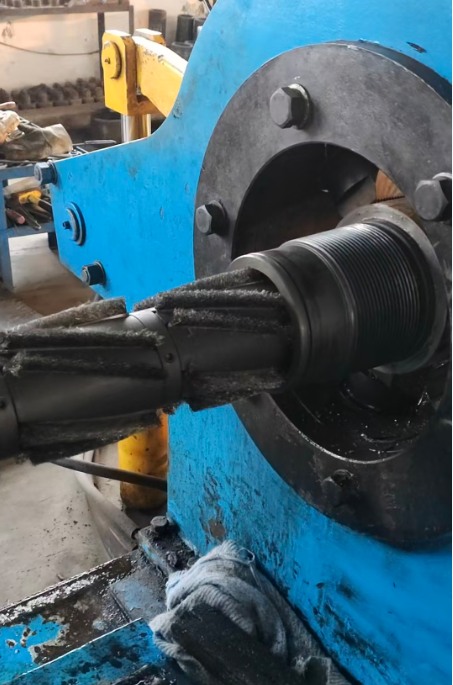
\includegraphics[height=8.0cm]{figure/chapter3/part1-3in1/brush-pipe-test-1.png}}
	\hfill
	\subfloat[毛刷短节在管内往复活动]{%
	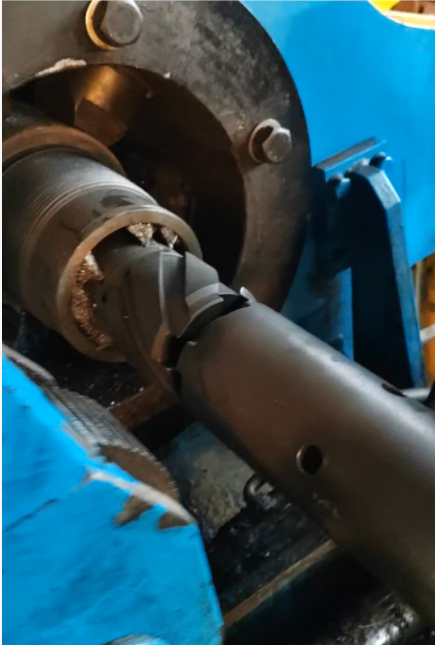
\includegraphics[height=8.0cm]{figure/chapter3/part1-3in1/brush-pipe-test-2.png}}
	\caption{毛刷刮管器通过性试验}
	\label{fig:3in1_brush_test}
\end{figure}

由图\ref{fig:3in1_brush_test}可见，毛刷短节装配后能够顺利进入试验管段，并在管内往复活动过程中与管壁保持接触。所测摩擦力可作为判断毛刷压缩量是否合适、工具在套管内是否易于遇阻的依据。

\subsubsection{脉冲器试验}

脉冲器试验采用打压泵打压。打压3\,min内，泵压波动范围为$0\sim4$\,MPa；当排量达到300\,L/min时，脉冲器开始振动，实测振动频率为$15\sim20$\,Hz，工作状态如图\ref{fig:3in1_pulser_test}所示。

\begin{figure}[htbp]
	\centering
	\subfloat[脉冲器试验台架安装]{%
	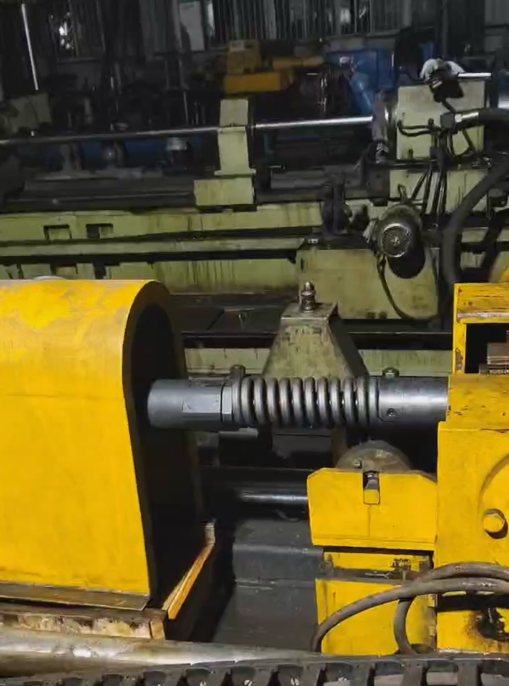
\includegraphics[height=8.0cm]{figure/chapter3/part1-3in1/pulser-test-bench-1.png}}
	\hfill
	\subfloat[脉冲器出水振动状态]{%
	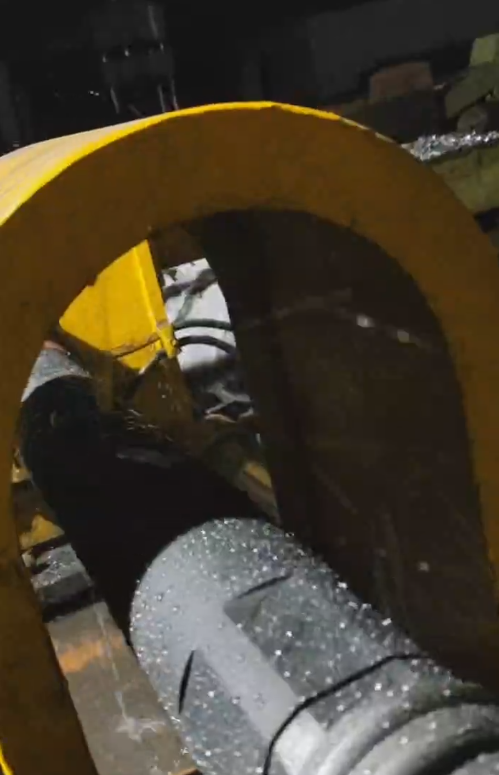
\includegraphics[height=8.0cm]{figure/chapter3/part1-3in1/pulser-jetting-test.png}}
	\caption{脉冲器试验状态}
	\label{fig:3in1_pulser_test}
\end{figure}

脉冲器出厂前单独试验的测试数据见表\ref{tab:3in1_pulser_factory}。

\begin{table}[htbp]
    \centering
    \caption{脉冲器出厂试验数据}
    \label{tab:3in1_pulser_factory}
    \small % 列数较多，适当缩小字号，避免超出正文版心
    \setlength{\tabcolsep}{3pt}
    \renewcommand{\arraystretch}{1.4}
    \begin{tabular*}{\textwidth}{@{\extracolsep{\fill}}ccccccc@{}}
        \toprule % 顶线
        型号 & 名称 & \begin{tabular}[c]{@{}c@{}}喷嘴直径\\ ($\times$2, mm)\end{tabular} & 
        \begin{tabular}[c]{@{}c@{}}压力\\ (MPa)\end{tabular} & 
        \begin{tabular}[c]{@{}c@{}}流量\\ (L/min)\end{tabular} & 状态 & 备注 \\
        \midrule % 栏目线
        \multirow{3}{*}{MCQ105} & \multirow{3}{*}{4\,1/8\,英寸脉冲短节} & 3.175 & 2 & 200 & 未震动 & 脉冲1 \\
        & & 3.175 & 6 & 420 & 开始震动 & 脉冲2 \\
        & & 3.175 & 8 & 480 & \begin{tabular}[c]{@{}c@{}}弹簧压并不回弹\\ （泄压后回弹）\end{tabular} & 脉冲3 \\
        \bottomrule % 底线
    \end{tabular*}
\end{table}

由表\ref{tab:3in1_pulser_factory}可见，出厂试验时泵压在$6\sim8$\,MPa范围内脉冲器可保持低频往复运动；当泵压大于8\,MPa时，弹簧被压并而无法回弹。分析认为，其原因可能为喷嘴直径偏小，活塞滑过喷嘴孔后喷嘴泄流泄压不明显，弹簧所受作用力减小幅度不足，因而无法复位。

针对上述问题，脉冲器的优化方案为：更换大口径喷嘴，并加大弹簧预压力，保证泄压过程明显、回弹弹力充足。

此外，本次测试中脉冲器在300\,L/min时即已起振，低于出厂单独试验的起振排量（420\,L/min），两者试验条件（管串组合与背压）不同，其对应关系尚需在整机试验中进一步标定。

\subsubsection{液压刮管器试验}

测试前先在井口投球，钢球直径为$\phi$28\,mm。使用泵车打压，泵压升至15\,MPa时刮刀无动作，停泵泄压；随后将泵压升至17\,MPa，刮刀张开，张开行程约8\,mm。停泵后泵压下降至0\,MPa，刮刀未能自行回收，拆下管线后刮刀才回收，刮刀状态如图\ref{fig:3in1_scraper_test}所示。

\begin{figure}[htbp]
	\centering
	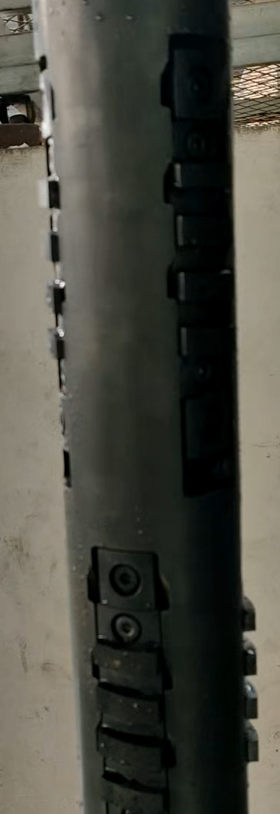
\includegraphics[width=3.4cm]{figure/chapter3/part1-3in1/hydraulic-scraper-blades.png}
	\caption{液压刮管器刮刀状态}
	\label{fig:3in1_scraper_test}
\end{figure}

液压刮管器出厂前静液压试验的测试数据见表\ref{tab:3in1_scraper_factory}。

\begin{table}[htbp]
    \centering
    \caption{液压刮管器出厂试验数据}
    \label{tab:3in1_scraper_factory}
    \small % 列数较多，适当缩小字号，避免超出正文版心
    \setlength{\tabcolsep}{3pt}
    \renewcommand{\arraystretch}{1.4}
    \begin{tabular*}{\textwidth}{@{\extracolsep{\fill}}ccccccc@{}}
        \toprule % 顶线
        型号 & 名称 & \begin{tabular}[c]{@{}c@{}}激活钢球\\ (mm)\end{tabular} & 
        \begin{tabular}[c]{@{}c@{}}激活压力\\ (MPa)\end{tabular} & 
        \begin{tabular}[c]{@{}c@{}}剪切螺钉\\ 数量\end{tabular} & 
        \begin{tabular}[c]{@{}c@{}}张开外径\\ (mm)\end{tabular} & 备注 \\
        \midrule % 栏目线
        YYGG105 & 4\,英寸液压刮管器 & $\phi$28 & 40 & 12（钢） & 130 & 刮壁器1 \\
        \multicolumn{2}{c}{出厂设置} & --- & 20 & 8（铜） & --- & 刮壁器2 \\
        \bottomrule % 底线
    \end{tabular*}
\end{table}

第一次静液压试验采用钢制剪钉，投球后泵压达到40\,MPa时剪钉剪断、刮刀张开；此后改用铜制剪钉，剪切压力为20\,MPa$\pm$2\,MPa。第二个$\phi$32\,mm钢球仅在需要强制回收刮刀时投放，投放后水眼封闭，因此可将上球座改为滑套结构，使投球后水眼保持畅通。

东营试验基地试验中，投球后泵压升至17\,MPa时销钉即已剪断，但刮刀未完全伸出；刮刀完全张开所需泵压≥2\,MPa，此时泵压是否达到要求尚不确定。停泵后刮刀未收回，可能为刮刀滑槽内有异物或机械卡滞所致；卸掉水龙带时工具产生轻微振动，滑槽恢复顺畅后刮刀才顺利回位。

\subsubsection{旋转喷头试验}

试验使用泵车供液。先将排量调至0.15\,m$^3$/min，以较低排量循环，旋转喷头出水但未旋转；随后逐步提高排量，最高升至0.45\,m$^3$/min，旋转喷头仍只出水而不旋转，停泵，测试结束。旋转喷头试验状态如图\ref{fig:3in1_nozzle_test}所示。

\begin{figure}[htbp]
	\centering
	\subfloat[试验前喷头与工具串连接]{%
	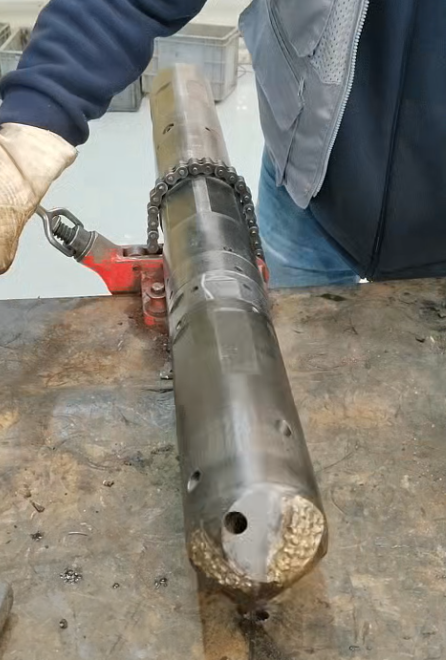
\includegraphics[height=8.0cm]{figure/chapter3/part1-3in1/rotary-nozzle-makeup.png}}
	\hfill
	\subfloat[试验中喷头射流状态]{%
	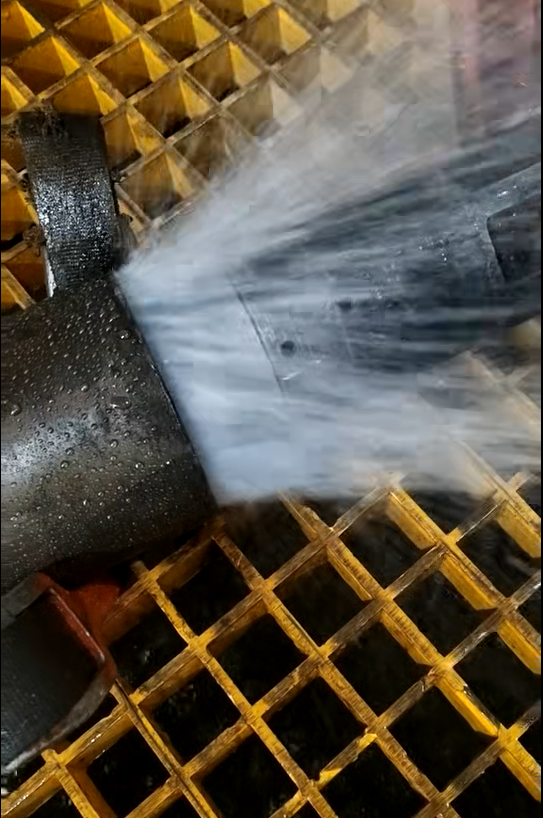
\includegraphics[height=8.0cm]{figure/chapter3/part1-3in1/rotary-nozzle-jetting.png}}
	\caption{旋转喷头试验状态}
	\label{fig:3in1_nozzle_test}
\end{figure}

旋转喷头出厂试验数据见表\ref{tab:3in1_nozzle_factory}。

\begin{table}[htbp]
    \centering
    \caption{旋转喷头出厂试验数据}
    \label{tab:3in1_nozzle_factory}
    \small % 列数较多，适当缩小字号，避免超出正文版心
    \setlength{\tabcolsep}{3pt}
    \renewcommand{\arraystretch}{1.4}
    \begin{tabular*}{\textwidth}{@{\extracolsep{\fill}}cccccccc@{}}
        \toprule % 顶线
        型号 & 名称 & \begin{tabular}[c]{@{}c@{}}喷嘴直径\\ (mm)\end{tabular} & 
        \begin{tabular}[c]{@{}c@{}}喷嘴\\ 数量\end{tabular} & 
        \begin{tabular}[c]{@{}c@{}}工作压力\\ (MPa)\end{tabular} & 
        \begin{tabular}[c]{@{}c@{}}工作流量\\ (L/min)\end{tabular} & 
        \begin{tabular}[c]{@{}c@{}}转速\\ (r/min)\end{tabular} & 备注 \\
        \midrule % 栏目线
        XZPT105 & 4\,1/8\,英寸旋转喷头 & 3.175 & 7 & $\ge2$ & $\ge350$ & $10\sim300$ & 旋转喷头1 \\
        \multicolumn{2}{c}{二次试验工具串} & 3.175 & 5（2个未装） & $\ge3$ & $\ge450$ & $10\sim300$ & 旋转喷头3 \\
        \bottomrule % 底线
    \end{tabular*}
\end{table}

旋转喷头单独试验时，排量达到$350\sim400$\,L/min即开始旋转，此时泵压约为2.2\,MPa；接入刮刀与脉冲器后，管内压降发生变化，拆掉2个喷射喷嘴并提高排量、使泵压不低于3\,MPa后，喷头才开始转动。本次东营基地试验中喷头未能转动，可能与上部工具压耗过大有关。试验过程中应保证泵压不低于3\,MPa，或将旋转喷头头部下入套管内，以增大喷射孔的反冲力矩。

\subsubsection{试验结论与改进措施}

综合各模块的试验结果，可得如下结论：

\begin{itemize}
	\item 毛刷刮管器装配后可通过$\phi$114\,mm试验管段并往复活动，毛刷与管壁保持接触，满足入井刮刷对通过性的要求；
	\item 脉冲器在300\,L/min、泵压波动$0\sim4$\,MPa条件下可正常起振，振动频率为$15\sim20$\,Hz；但当泵压大于8\,MPa时弹簧压并不回弹，需通过更换大口径喷嘴、加大弹簧预压力予以改进；
	\item 液压刮管器在15\,MPa时未动作、17\,MPa时刮刀张开，张开行程约8\,mm；停泵后刮刀不能自行回收，需拆卸管线后才能回位，反映剪钉剪切压力与刮刀回位机构仍需优化；
	\item 旋转喷头单独试验时，在$350\sim400$\,L/min、2.2\,MPa条件下即可旋转；接入刮刀与脉冲器后需在泵压不低于3\,MPa时才转动；东营基地试验中因上部压耗过大未能转动，需在整机联调中重新匹配排量与压耗。
\end{itemize}

针对试验中暴露的问题，后续将从喷嘴通径、弹簧预压力、剪钉配置与球座结构以及喷头压耗匹配等方面对工具进行改进，并在整机联调中复测验证。

\subsection{“三合一”工具应用效果室内测试评价工艺}
\label{sec:eval-3in1}

\subsubsection{整套工具运行检查}
按实际连接顺序装配毛刷刮管器、液压刮管器、脉冲发生器和旋转喷头，改变供液流量，检查是否产生脉冲、喷头是否连续旋转、刮板能否张开和收回。记录压力随时间变化的曲线、喷头转速和刮板动作，确认各部分连接后能否正常工作，并检查整套工具能否通过相应管段。

压力变化和喷头转速用于检查工具运行情况；管壁清洁和筛孔疏通效果按下述试验评价。

\subsubsection{套管和筛管清洁试验}
使用带附着物的套管或已经堵塞的筛管，在规定流量、移动速度和清洁时间下运行工具，称量清洁前后的附着物，并拍摄管壁和筛孔残留。附着物清除比例为清洁前质量减去残留质量，再除以清洁前质量并乘以100\%；初始质量须大于零，前后称量的干燥或含液条件一致。比较参数时保持初始污染程度一致。

将筛管装入密封套筒，封住端部绕流通道，使液体穿过过滤层。在相同液体、温度、流向及筛管内外压差下，测量洁净、堵塞及清洁后的筛管流量，流量恢复比例按式\eqref{eq:eval-screen}计算：
\begin{equation}
	\eta_f=\frac{Q_1-Q_b}{Q_0-Q_b}\times 100\%
	\label{eq:eval-screen}
\end{equation}
式中，$\eta_f$--筛管流量恢复比例，\%；$Q_0$、$Q_b$、$Q_1$--分别为洁净、堵塞和清洁后的筛管流量，L/min，且$Q_0>Q_b$。该比例表示堵塞所损失流量的恢复程度，三次流量与计算结果一并列出。

单独计量穿过筛管过滤层的液体，清洁循环排量另列；检查筛管破损和绕流泄漏。

\subsubsection{耐用性试验}
在规定流量和运动条件下持续运行，定期停机检查，累计时间、刮刷行程和刮板张开收回次数。在相同位置测量喷嘴孔径增大量、刮板刃口尺寸减小量及刷丝缩短量，记录脉冲消失、喷头停转和刮板收回异常。

用初始污染或堵塞程度相当的新管段，按最初条件复测附着物清除比例或筛管流量恢复比例，与初始值的差以百分点表示。结合零件磨损及清洁效果随累计时间的变化评价耐用性。

\subsubsection{作业效率试验}
对初始附着物相当的套管组或堵塞流量相当的筛管组，分别清洁不同时间，测量清除比例或流量恢复比例。计时从脉冲、喷头及刮刷按规定方式工作起，至清洁结束；拆装、称量和流量测量时间另列。

达到规定清除比例或流量恢复比例所需时间，取达到要求的试验组中最短时间。套管试验以清除质量除以清洁分钟数，计算每分钟清除量（g/min）。结合效果与时间，比较流量及移动速度对效率的影响。
